\documentclass[11pt]{article}
\usepackage{todonotes}
\usepackage{fullpage}
\usepackage{amsmath}
\usepackage{setspace}
\usepackage{listings}
\usepackage{verbatim}
\usepackage{algpseudocode}
\usepackage{algorithm}
\usepackage{caption}
\usepackage{graphics}
\algblockdefx[IF]{If}{EndIf}[1]{\algorithmicif\ #1}{\algorithmicend}
\algblockdefx[WHILE]{While}{EndWhile}[1]{\algorithmicwhile\ #1}{\algorithmicend}
\algblockdefx[FOR]{For}{EndFor}[1]{\algorithmicfor\ #1}{\algorithmicend}
\algblockdefx[FUNCTION]{Function}{EndFunction}[2]{\algorithmicfunction\ \textsc{#1}(#2)}{\algorithmicend}
\usepackage{galois}
\usepackage{tikz}
\usepackage{varwidth}
\usetikzlibrary{positioning}
\usetikzlibrary{arrows.meta,bending,automata}
%\usepackage{pxfonts}
\usepackage[urw-garamond]{mathdesign}
\usepackage{multicol}
\usepackage[T1]{fontenc}
\lstdefinelanguage{julia}{
  basicstyle=\small\ttfamily,
  basewidth=0.5em,
  showspaces=false,
  showstringspaces=false,
  keywordstyle={\textbf},
  morekeywords={if,else,elseif,while,for,begin,end,quote,try,catch,return,local,abstract,function,stagedfunction,macro,ccall,finally,typealias,break,continue,type,global,module,using,import,export,const,let,bitstype,do,in,baremodule,importall,immutable},
  escapeinside={~}{~},
  morecomment=[l]{\#},
%  commentstyle=\textsf,
  commentstyle={},
  morestring=[b]",
}
\newcommand{\F}{\mathcal{F}}
\renewcommand{\P}{\mathcal{P}}
\newcommand{\eps}{\varepsilon}
\renewcommand{\kappa}{\varkappa}
\renewcommand{\phi}{\varphi}
\newcommand{\D}{\Diamond}
\newcommand{\uD}{\underline{\Diamond}}
\newcommand{\UD}{\overline{\Diamond}}
\renewcommand{\S}{\mathcal{S}}
\newcommand{\oS}{\overline{\mathcal{S}}}
\newcommand{\dS}{\delta\mathcal{S}}
\newcommand{\ra}{\rightarrow}
\DeclareMathOperator{\lfp}{lfp}
\DeclareMathOperator{\dom}{dom}
\DeclareMathOperator{\idom}{idom}
\DeclareMathOperator{\children}{children}
\DeclareMathOperator{\parent}{parent}
\DeclareMathOperator{\dest}{dest}
\DeclareMathOperator{\src}{src}
\DeclareMathOperator{\roots}{roots}
\DeclareMathOperator{\DF}{DF}
\DeclareMathOperator{\IDF}{IDF}
\title{\vspace{-6ex}A modular abstract interpreter for Julia \\ MPRI internship report}
\author{Oscar Blumberg, supervised by Prof.\@ Alan Edelman, MIT}
\date{2015}
\begin{document}
\onehalfspacing
\maketitle

\thispagestyle{empty}
\vspace{1.5ex}
\subsection*{General context}

Julia\cite{julia-paper,julia-web} is a dynamically typed, JIT compiled, programming language implementation with an emphasis on generic programming through a powerful and ubiquitous symmetric, dynamic multiple dispatch mechanism. It achieves superior run-time performance by relying heavily on static analysis and aggressive code specialization. It is meant to provide a tool for scientific computations that is both familiar and fast enough for this demanding usage. The Julia compiler also provides a range of metaprogramming and code generation techniques to the advanced user.

Efforts into optimizing dynamic languages date back to Common Lisp tradition\cite{cl}, and more recently the sizable effort into making various JavaScript engines high performance\cite{js-trace}. Julia has the interesting advantage of having been designed from the ground up to be a good analysis target and, while being dynamic, avoids pathological behavior patterns that are very hard to infer statically.

\subsection*{Studied problem}

Most optimizations in the Julia compiler are done by the LLVM\cite{llvm} library in the backend. LLVM is a widely used, production-grade compiler and generally generates excellent machine code. However, its intermediate representation operates at an abstraction level comparable to that of C.

Some program optimizations would be better performed on the much higher level semantic that Julia code exhibits earlier in the compilation pipeline. The backend has to deal with additional complexity due to the integration between the generated code and the various run-time systems: dynamic memory allocation, garbage collection, dynamic dispatch call-sites, ...

At the Julia level, all those operations are implicit and the allowed behaviors are much more restricted: it has no interior pointers, no stack escape, memory operations cannot trap, type-punning is forbidden, the list goes on. It makes some analysis much easier, alias and shape analysis being good examples. \todo[inline]{I like this list... maybe can expand on how this is also easier for abstract interpretation later in this report}


\subsection*{Proposed contributions}

As the main project of this internship, an extensible static analysis library for Julia was started. Dubbed the \emph{Green Fairy}, it is written itself in Julia. The exposed interface is that of an abstract interpreter, providing an intuitive model for program behavior inference.

It uses a spatially sparse representation of the interpreter state enabling scalability across large programs. The main value domain is an extensible generic implementation of the reduced product construction, making it reasonably easy to extend it with new models.

It also features a work-in-progress interprocedural flow-sensitive shape analysis, based on static shape graphs\cite{ssc}. The shape analysis uses a sparse representation as well, and an optimistic but conservative model of aliasing information for the unknown parts of the heap that allows it to treat gracefully the usual problem of the cost of context sensitivity. It is able to track bounded allocation lifetimes across loop iterations precisely, opening up the possibility of interesting static garbage collection optimizations.

\subsection*{Arguments supporting their validity}

The implementation is available as an ongoing work at \cite{gf-web}. It is already capable of applying both value-level (currently constant propagation and type inference) and shape analysis to a significant body of Julia code.
It succeeds in demonstrating our ideas on a \emph{non-toy} real world language, including its more exotic and idiosyncratic features.
We hope to integrate our work into the main compiler in the coming year.

\subsection*{Future work}

Besides tying up the various technical loose ends and improving the non-algorithmic bottlenecks of the implementation, we have several goals for the future of this project.

A consequent amount of technical work has to be done to make the later stages of the compiler modular enough that the friction in taking advantage of new information from the analysis becomes much lower \todo{Wordy}. In particular, we plan to implement optimizations using the shape analysis to provide precise no-escape information that will allow memory reuse and stack allocation, greatly reducing the load on the garbage collector and the dynamic allocator.

In the longer term, the natural extension to this work is to devise an intuitive interface that makes it possible for users to extend the abstract state of the interpreter with domain-specific informations. We hypothesize that there is a large class of optimizations that are hard-to-impossible to teach a compiler using only knowledge of the language's semantic, but are fairly easy to formulate once more information is given about specific data structures and idioms in use. \todo[inline]{What optimizations do you think belong in this class?}

Those points are developed further along in the report.

\break
\begin{comment}
\section*{What is abs int (??!!)}

[probably some note somewhere on how AI is a different, more general, vocabulary for dataflow but is really the same idea]
[expand a bit more ? it's already quite long for pedestrian stuff]


At its core, abstract interpretation is a mathematical framework intended to formally describe a large class of static program analysis.
It provides a language and generic tools to prove their soundness.
The following is intended as a light and informal explanation. The reader familiar with this concept can safely skip it. For a complete exposition, we refer to the seminal paper introducing abstract interpretation\cite{absint-cousot}.

Static analysis is the idea of deriving provably true information about the \emph{run time} behavior of a program in a finite -- and reasonable -- amount of time.
The usage of static analysis is extremely broad and ranges from the most basic compiler optimization to a rich zoo of safety checkers.
A typical analysis assumes a class of hypotheses about a computer program's inputs and interactions with the outside world, and concludes some assertions
about every possible execution of said program.

\paragraph{State space} Computational systems are classically described as a dynamical process over some state space $\S$, with the process itself described by a transfer operator $T:\S\to\S$. We want $\S$ to describe the behavior of the program completely. A first choice could be to make $\S$ the set of possible execution traces, that is, each state describes the whole past of a particular execution of the program up to a certain point. The transfer is simply completing a specific trace, adding its next step to it.

It is however useful to consider \emph{non-deterministic} systems, even in the study of fully deterministic programs, as it provides a way to model unknowns. For example, a program reading some integer value from the outside world can be modeled as non-deterministically choosing an integer. A trace that ends by doing such an unknown operation has several valid continuation traces, possibly one for each integer value. \todo[inline]{You've given an example, but it doesn't motivate why modeling deterministic systems nondeterministically is useful.}

To represent the unknown states, let elements of $\S$ be sets of execution traces. They are naturally ordered by set inclusion, forming a complete lattice.
In fact, we can think of this order as a measure of the information given by the knowledge that a specific trace lives in one of those sets.
We can sketch static analysis in the following way: given some information $\sigma\in\S$, about the state of a program, what can be deduced about
all the reachable states from $\sigma$ in a reasonable amount of time?

\todo[inline]{What is a simpler, if less precise, answer to this question? Starting by giving the most precise answer implies that it is somehow not the easiest answer.}
The most precise answer to this question is the smallest element of $\S$ that both contains $\sigma$ and is stable by $T$. Let's call it $\lfp_\sigma(T)$. This element is exactly the set of all possible traces of executions starting inside $\sigma$. The name lfp stands for least fixed point and in our case we can express it as
\[ \lfp_\sigma(T) = \sigma \cup T(\sigma) \cup T^2(\sigma) \cup \dots \]
Computing it is not possible: it is equivalent to simulating every execution of the program. Halting problem aside, it is obviously quite impractical. However, any upper bound of $\lfp_\sigma(T)$ gives us \emph{some} information on the reachable states. Abstract interpretation is a way of describing this process of purposefully losing information. This over-approximation -- or \emph{abstraction} -- of the state space, lowers the precision of the result but makes it computable, both theoretically and realistically.

\paragraph{Abstraction} We will model this voluntary loss by an abstraction function $\alpha:\S\to\oS$ landing in a lattice $\oS$ of our choosing that will approximate $\S$. Given a state $\sigma$, we think of $\alpha(\sigma)$ as the amount of information we want to retain about $\sigma$. We also need a \emph{concretization}, $\gamma:\oS\to\S$, that brings us back to the original state space giving a meaning to elements of $\oS$.\todo[inline]{Clearly if abstraction results in information loss, then $\gamma$ is not unique. Do you mean to pick one possible $\gamma$, or consider the set of all possible images $\gamma(\overline{\sigma})$?} \todo[inline]{The jargon 'morphism' and 'Galois connection' suddenly appear with no introduction.} The property for this pair of morphisms $\alpha,\gamma$ to be a sound abstraction is that $\S\galois{\alpha}{\gamma}\oS$ is a Galois connection, i.e., for any $\sigma\in\S$ and $\overline{\sigma}\in\oS$, we have
\[ \sigma \leq \gamma(\overline{\sigma}) \iff \alpha(\sigma) \leq \overline{\sigma} \]
\todo[inline]{Motivate why the definition of such a construct is useful.}
To give a concrete example of such an abstraction -- and avoid breaking with tradition \todo{what is the purpose of this clause?} -- consider $\S = 2^{\mathbb{N}}$ and $\oS = \{\bot,-,0,+,\top\}$ where we want to approximate any set of integers by its sign information. The pair of mappings \todo{but you already used "morphism" for this idea} would be the following:

\hfill

\begin{minipage}{0.4\linewidth}
\[
\gamma:
\begin{cases}
\hfill \bot \hfill \mapsto & \emptyset \\
\hfill \top \hfill \mapsto & \mathbb{N} \\
\hfill -   \hfill \mapsto & \left]-\infty,0\right[ \\
\hfill +   \hfill \mapsto & \left]0,+\infty\right[ \\
\hfill 0   \hfill \mapsto & \left\{0\right\} \\
\end{cases}
\]
\end{minipage}
\quad
\begin{minipage}{0.4\linewidth}
\[
\alpha(\sigma) =
\begin{cases}
\bot \hfill & \text{if } \sigma = \emptyset \\
 0   \hfill & \text{if } \sigma = \left\{0\right\} \\
 -   \hfill & \text{if } \forall x\in\sigma, x < 0 \\
 +   \hfill & \text{if } \forall x\in\sigma, x > 0 \\
\top \hfill & \text{otherwise} \\
\end{cases}
\]
\end{minipage}

\hfill

In this setup, we have $\alpha(\left\{1,3\right\}) = +$ and $\alpha(\left\{-1,3\right\}) = \top$. This abstraction is able to remember that the first set only has positive elements but cannot give any information about the second set.

\paragraph{Transfer} To analyze a program, we will compute in $\oS$ instead of $\S$, making it \todo[inline]{what is it? Ambiguous ``it'' is a very common problem in technical writing.} tractable. The missing piece is now to translate the program's semantics into the abstracted state space. We will call this abstracted transfer morphism $\overline{T}:\oS\to\oS$ \todo[inline]{Unclear "this" - it took me several readings to realize that you do actually want the endomorphism over $\oS$. The next three sentences describe the construction of $\overline T$ but the discussion is of the explicit projection $\oS\to\S$. confusing...}. The most precise possible choice for $\overline{T}$ is given by
\[ \overline{T}_{\text{exact}} = \alpha\circ T\circ \gamma \]
however this is not a practical definition since it involves computing in $\S$ \todo{"Which is what we want to avoid in the first place"?}. Nevertheless, any upper bound of $\overline{T}_{\text{exact}}$ for the pointwise order will still give rise to a sound abstraction of $T$, albeit less precise. It \todo{what?} depends on the choice of $\alpha,\gamma$ \todo{Spell out Galois connection?} whether it is or not possible to express $\overline{T}_{\text{exact}}$ in a computable manner.

Once a sound $\overline{T}$ is chosen, we can compute an approximation of the program's behavior by the identity
\[ \lfp_\sigma(T) \leq \gamma(\lfp_{\alpha(\sigma)}(\overline{T})) \]
In other words, we can \emph{execute} the program in $\oS$ using $\overline{T}$, instead of in $\S$ using $T$, and use the resulting information with the guarantee that the actual program behavior is described by the abstract behavior.

As an example, consider the following program in a toy imperative language with a single variable:

\begin{algorithmic}[1]
\State $x = 1$
\While{$x < 1000$}
\State $x = x+1$
\EndWhile
\end{algorithmic}


Suppose we want to prove that $x$ has to be positive by the time the program ends. The first abstraction step is to trim the large state space of traces into a more manageable domain. We will collapse each trace into its last step in the form of a tuple $\left(pc,x:v\right)$ where $pc$ is the program point and $v$ the value of $x$. One abstract state of this first domain can be seen as a mapping from program control points to sets of possible integers. In our case, the result after program execution -- when the fixed point of $\overline{T}$ is reached -- would be
\[
\begin{cases}
1 \mapsto & x:\{1\} \\
2 \mapsto & x:\{1, \dots, 999\} \\
3 \mapsto & x:\{2, \dots, 1000\} \\
4 \mapsto & x:\{2, \dots, 1000\} \\
\end{cases}
\]
but computing this result would require up to a thousand iterations. If instead we compute the values of $x$ in the sign domain, the fixed point is reached in a single loop iteration because the sign of $x$ does not change. Moreover, we would still be able to conclude since we were only interested in the resulting sign of $x$ in the first place.

Although this trivial example only deals with abstracting values, a fundamental trait of abstract interpretation is that the whole state of the program -- or rather its interpreter -- can be abstracted in the same framework. This allows us to treat uniformly, at least on the proof level, the loss of precision due to value approximation and various other simplifications, such as context/path/flow-insensitivity or the choices of modeling for the program heap.


\paragraph{Product domains} Having a generic language also opens the opportunity for generic constructs, such as the reduced product. Given two abstract domains $D_1$ and $D_2$, we want to build a combination of those that carries at least as much information. The first natural choice could be the Cartesian product; however, there is no advantage in computing in $D_1\times D_2$ compared to running two separate analysis. We can instead, given two reduction maps $r_1:D_1\times D_2\to D_1$ and $r_2:D_2\times D_1\to D_2$, form the so-called reduced product $D_1 \otimes D_2$ under some soundness conditions. [note: same as fibered product in the category associated to the order] Elements $s_1\otimes s_2$ of $D_1 \otimes D_2$ satisfy the property that $r_1(s_1,s_2) = s_1$ and $r_2(s_2,s_1) = s_2$. Intuitively, $r_1$ and $r_2$ provide cross domain intersection -- or meet. That is, they must satisfy \todo{all of the following criteria?}
\begin{align*}
r_1(s_1,s_2) \leq s_1~\text{and}~ \gamma_1(r_1(s_1,s_2)) \leq \gamma_2(s_2) \\
r_2(s_2,s_1) \leq s_2~\text{and}~ \gamma_2(r_2(s_2,s_1)) \leq \gamma_1(s_1)
\end{align*}
The reduced product formalizes the sharing of information between separate abstract domains, and is central to the modularity of our implementation.

As with all elegant formalisms, abstract interpretation provides a good way to structure one's thoughts. Here, about families of static analysis. \todo{fragment} By extension, it also points towards a good way to structure the analyzer itself in a composable way.
\end{comment}
\section*{Julia}
Julia has a dynamically-typed semantic. The execution model is that of a typical imperative language : impure and call by value. It is entierly built around the concept of generic functions.
\paragraph{Type system} dedede

\paragraph{Generic functions} A function in Julia is in fact a collection of methods, partially ordered by their signature types as a sub-lattice of the type lattice\cite{julia-paper}.
The dispatch mechanism is dynamic -- albeit statically inferred in many cases -- and is symmetric in all the arguments: the most specific method will be called at run-time depending on the argument types.
It is ensured that for any argument type there exists a well defined least upper bound in the sub-lattice.
More details about Julia's generic functions can be found in \cite{julia-paper,jeff-phd}.

\paragraph{Memory model} At the specification level, Julia objects are tagged memory cells living in an infinite heap. Each has a finite set of numbered mutable fields, possibly pointing to other objects. The language relies on automatic memory management to fit in a physical finite heap.
The current implementation uses a tracing garbage collector.

\paragraph{Compiler} The main analysis performed on Julia code by the compiler is an interprocedural flow-sensitive type inference. It is followed by an inlining pass and several ad-hoc peephole optimization. The last step is to generate LLVM intermediate representation while using the infered types to remove as much of the dynamic semantic as possible.
This project addresses the limitation that the only static information computed on high level Julia code today is in the type lattice.

\todo[inline]{Say more}

\section*{Green Fairy}

The Green Fairy provides a generic framework that computes the fixed point of user-provided abstractions over a Julia program.
The library handles the control flow semantics and presents itself as an extensible interpreter : users enrich the abstract machine's state with custom abstractions.

We provide a set of generic basic blocks to construct those state extensions.
The most common one is a non-relational variable analysis over any value domain.
It can be used jointly with the supplied parametric reduced product\cite{redprod} implementation, allowing for the implementation of cooperative behavior between different domains.
We will start by giving a short and simple example of its usage.

\subsection*{Interval example}
Follows an implementation of the classical example of abstract domain: the (closed) numeric interval.
\begin{singlespace}
\begin{lstlisting}[language=julia]
immutable Interval{T} <: Lattice
    lo :: T
    hi :: T
end

bot{T}(::Type{Interval{T}}) = Interval(typemax(T),typemin(T))
top{T}(::Type{Interval{T}}) = Interval(typemin(T),typemax(T))
isbot(x::Interval) = x.hi < x.lo

<=(x::Interval,y::Interval) = isbot(x) || y.lo <= x.lo && x.hi <= y.hi
join{T}(x::Interval{T},y::Interval{T}) = Interval(min(x.lo,y.lo), max(x.hi,y.hi))

function meet_ext{T}(x::Interval{T}, c::Const)
    !istop(c) && isa(c.v,T) || return x
    x.lo <= c.v <= x.hi && return Interval(c.v, c.v)
    bot(Interval{T})
end
\end{lstlisting}
\end{singlespace}

This domain is parametric over any ordered numeric types having an upper and lower bound. Defining a method for \verb~isbot~ is necessary since there are multiple representation of $\bot$.

The \verb~meet_ext~ function is the product domain reduction function. In that case we express that the knowledge that a value is constant can reduce an interval to a single point or $\bot$ depending on the particular value. We are free to add other method definitions to this function to increase precision using information from other domains than \verb~Const~. This modelization of the reduced product relies on multiple dispatch to easily provide extension points : the user can seamlessly provide reduction functions for any pair of domains, possibly defined by someone else.
%\todo[inline]{From this description, here sounds like a good place to mention that meet\_ext is a generic function and can be extended with multimethods without the need to give the new definitions new names. And it's worth saying why the multimethod approach is more elegant here, after putting this entire section after the one about Julia semantics.}

Describing transfer functions is also straightforward, as demonstrated by this simple example implementing the transfer for the addition on the interval lattice:
\begin{singlespace}
\begin{lstlisting}[language=julia]
function eval_call{T,V}(::Type{Interval{T}}, f::V, args::Vector{V})
    if f <= Const(Base.(+))
        intervals = map(v -> convert(Interval{T}, v), args)
        lbs, ubs = map(i -> i.lo, intervals), map(i -> i.hi, intervals)
        return Interval(sum(lbs), sum(ubs))
    end
    top(Interval{T})
end
\end{lstlisting}
\end{singlespace}
We can see that the arguments can be provided in different domain than that of intervals, requiring a \verb~convert~ call. This gives access to the full product to a transfer function, making it possible to use information from other domains in the computation.
%\todo[inline]{Is eval\_call a transfer function? It is unclear from the description. This paragraph describing the code is not a good place to mention generalities about what transfer functions can do. What is this specific transfer function doing that illustrates the general principle?}

Due to space constraints, we relegate to the appendix another example that demonstrates the construction of a \emph{finite disjunction} domain that is parametric over any other domain and can thus serve as a composable building block. It can be used to enhance precision while keeping the implementation simple and decoupled.
Those two examples illustrate the benefits of the pervasive use of ad-hoc polymorphism and multiple dispatch in Julia: it allows for the construction of reusable abstractions.

Several important opt-in features for value domains and their transfer functions were not described here for the sake of brevity. This includes fused join-comparisons, widening, participation in the dispatch machinery, the ability to control the propagation of values over function call boundaries, as well as state-altering actions such as exception raising or heap operations.

\todo[inline]{Insisit more on modularity, maybe make a new section}

\subsection*{IR}

Our interpreter operates on a low-level dialect of Julia source code.
We will give here a simplified description of this internal representation.

A function is a control graph composed of extended basic blocks (EBB). Their defining property is to have a single control flow entry point as their head. Each one contains a linear succession of branches and variable assignments to literals and function calls.

Our implementation deals with most of the current Julia semantic.
We will leave out some of those features because while they require additional work, they are not directly relevant to this report. This includes
\begin{itemize}
\item Exception handling. Even though special care was taken to handle it with complete precision (assuming of course precise throw-site information).
\item Closure capture.
\item Function calls with variable number of arguments, or ``splatting''.
\end{itemize}

\todo[inline]{where put this}
Generic functions have interesting repercussions on analysis strategies. Since virtually every function call is indirect, not knowing the argument types can lead to a combinatorial blowup of code to explore in an interprocedural analysis, leading to widening and more precision loss. It is therefore often worth to trade performance for precision as long as it can keep types fully known\cite{jeff-phd}.

\section*{Analysis sparsity}
%\todo[inline]{I find this section very heavy and hard to read. There are a lot of details without much context of why I should care about the details. Could use some examples of the types of sparsity and how you can compress the analysis by taking advantage of sparsity.}
The Green Fairy is oriented towards building flow-sensitive analysis, that is, it provides information dependent on the program point.
The advantage of flow sensitivity is in the precision gain, although it comes with a performance price compared to the more approximative flow-insensitive analysis.
There are different techniques to lower the cost of flow sensitivity.

A simple way to implement a flow-sensitive computation is to store a dense mapping of program points to interpreter state. It has the benefit of being oblivious to the structure of said state.
However, as the state or the analyzed program gets larger, there is a growing cost associated to the copying and comparison of those state atoms.
In the vast majority of cases, the states at two nearby program points are highly redundant and taking advantage of this redundancy can lead to consequent improvements in analysis performance. Exploiting this so-called \emph{spatial} sparsity of the state space is an important design point of our implementation.

There is another related kind of sparsity, that is sometimes called \emph{temporal}, where the analyzer benefits from knowledge of state dependencies to avoid recomputing transfer operators that only use unchanged subset of the state. It allows the interpreter to make results from computations flow directly into use sites.
In the current implementation we do not use temporal sparsity, mainly due to a combination of time constraints and soundness concerns, although care was taken to ensure the feasibility of this optimization in the future.
In the literature, the word \emph{sparse} without qualification usually refers to temporal sparsity but we will mostly discuss spatial sparsity here.

\subsection*{Non-relational}

We implemented a sparse representation of non-relational state that accommodates any user-defined domain for forward analysis in a transparent manner.
This representation \emph{does not} require use/def sites to be identified ahead of time, unlike the Static Single Assignment (SSA) transform or other techniques relying on pre-analysis\cite{sparse-nr}.
Furthermore, we present an extension of this idea to a relational domain, namely, the static shape graph heap model as introduced in \cite{ssc}.

\paragraph{Static single assignment form} The classical example of sparsity is the \emph{SSA} transform. If a program is in SSA form, any forward variable analysis can easily be both spatially and temporally sparse. Taking advantage of the SSA transform is a two phase process. A pre-analysis identifies dataflow dependencies of variable uses over definitions. Once done, those dependencies are made explicit in the source code by renaming variables and inserting explicit join operations ($\phi$ instructions). It enables the use of a flow-insensitive analysis while keeping the precision of a flow-sensitive one.

\begin{comment}
Let's assume that the abstract state of interest is, for each program point, a simple mapping $\text{Var}\to V$ from variable names to some unspecified abstract value domain. Since a single variable mapping can change from a program point to at most one of its successors, it is tempting to only store -- at most -- a single $(\text{name}\mapsto\text{value})$ tuple for each statement of the program. One can then reconstruct the value of any variable $v$ at any point, simply by walking the CFG backward looking for the latest $(v\mapsto *)$ update. This scheme unfortunately is not sufficient, since in the presence of a statement with multiple control predecessors -- in our case, the head of an EBB -- we have to explore all of them to join the different possible values of $v$ together.

SSA solves this problem by summarizing the information about the ``past'' of variables at control flow join points, in the form of virtual $\phi$ instructions that makes the dependency of the variable's value in the different incoming edges explicit. A simple example is:

\begin{minipage}[t]{0.20\linewidth}
\begin{lstlisting}[language=julia]
a = 0
if ?
    a = 3
else
    a = 2
end
out(a)
\end{lstlisting}
\end{minipage}
\begin{minipage}[t]{0.30\linewidth}
\null
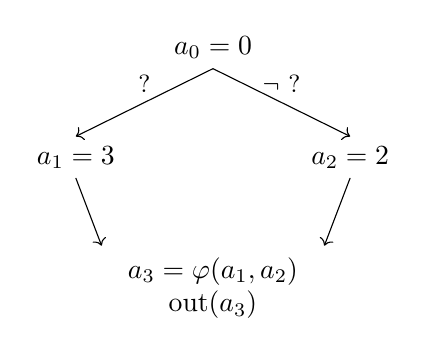
\begin{tikzpicture}[scale=.5]
\node[] (n0) {
  $a_0 = 0$
};
\node[below=of n0] (middle){};
\node[left=of middle] (n1) {
  $a_1 = 3$
};
\node[right=of middle] (n2) {
  $a_2 = 2$
  };
\node[below=of middle] (n3) {
\begin{tabular}{c}
  $a_3 = \phi(a_1, a_2)$ \\
  $\text{out}(a_3)$
\end{tabular}
  };
\draw (n0.south) edge[->] node[above]{\small ?} (n1.north)
      (n0.south) edge[->] node[above]{\small $\neg$ ?} (n2.north)
      (n1.south) edge[->] (n3.north west)
      (n2.south) edge[->] (n3.north east);
\end{tikzpicture}
\end{minipage}
\hfill
\end{comment}

\paragraph{Dominator tree} An important notion in the SSA transform is that of domination: we say that a program point $a$ \emph{dominates} another point $b$ if any path in the control flow graph from the root to $b$ has to go through $a$. The domination relation is a partial order on program points and is moreover a tree (every initial segment is well ordered). It is usually called the dominator tree. In our case, since every path to a program point has to go through the head of its containing EBB -- and all the points between the head and itself -- we will say that a program point dominates an EBB if it dominates its head. Given an EBB, the program point being its parent in the dominator tree is called the \emph{immediate dominator}.

The dominance frontier of a program point $a$, noted $\DF(a)$, is the set of EBB heads that, while not being dominated by $a$, have predecessors that are. $\DF(a)$ is the set of nodes that one has to pass through in order to, starting from $a$, leave its domination.
Following the usual convention, we note $\IDF(a) = \lfp_a\DF$ the iterated dominance frontier of $a$.

If a variable $v$ has two definitions at $a$ and $b$ respectively, the SSA form disambiguates between them by inserting $\phi$ nodes in a subset of $\IDF(a)\cap\IDF(b)$.
This set is an upper bound, because some of those $\phi$ may end up without any use. Computing the minimal $\phi$ placement is harder and requires a form of liveness analysis.
The advantage of the iterated dominance frontier is that $\IDF(a)$ only depends on $a$ and can be cached independently of the variable considered.

\paragraph{Sparse map} We take a slightly different approach from the usual SSA transform: we compute the same information but \emph{on the fly}. We assume that use sites of variables cannot be statically determined in advance without computing transfer functions.
It allows new use and definition sites to be discovered at an already processed program point in later iterations.
The main reason for this choice is to allow for other quantities than variable values to profit from the sparse infrastructure.
[examples]

Essentially, we are providing a generic sparse map implementation from an arbitrary set of names to any value domain.
It can be used to represent any non-relational internal interpreter state of the user's choice.

It is hence inefficient in our case to maintain the renaming property. Instead, when encountering an use, the interpreter walks the dominator tree upward to find the nearest definition.
This lookup is done following the tree spine, giving it an $O(\text{dominator tree depth})$ worst case complexity. In practice, the dominator tree is shallow and wide : in the Julia standard library (around 4MB of sources) the deepest dominator tree is of depth [?].

As for the implementation, we do not materialize $\phi$ instructions: they are kept out of band as a single compound summary information for each EBB head.
They can be efficiently dynamically updated when required by the discovery of new definitions.
We compute the dominator tree and frontiers using the algorithm described in \cite{domtree}.

We have not yet witnessed this process to be a bottleneck. Would it become the case, there are several ideas that could be implemented to lower its cost. The most obvious one being use-forwarding.
As an aside, the choice of EBBs for the program representation offsets the time spent doing this lookup in practice by making common dominator trees shallower.
It is not a worst-case improvement but a welcomed average constant factor gain.

% find somewhere to put this
%Another advantage of EBBs is that the dynamic addition of outbound control flow edges does not require node splitting. It is the case of exception throwing : it would degrade the sparsity of the CFG to conservatively assume that any statement can throw. Our interpreter generates new edges when a transfer function detects a possible raise.

\subsection*{Relational}

This structure cannot be readily used for relational domains, however we can extract an important insight from the non-relational case. We can think of the $\phi$ node living at an EBB's head as a summary of the state difference on any path between its immediate dominator and itself. It is less apparent in the case of a non-relational domain, since this difference is usually represented as an element of the domain itself, i.e., a small name-value mapping that only refers to changed names.

[good example + explanation of a generic translation]
[trash a bit \cite{sparse-nr} for saying relational in their title and only handling packed domains]

\section*{Shape analysis}

[todo some platitudes about shape analysis]

\subsection*{Local variables}
For a moment, we will ignore object fields and summary objects to concentrate on variable aliasing and its sparse structure. We will introduce those back later.
One of the fundamental insight of \cite{ssc} is in the scheme used to describe abstract heap locations.
The abstract address of an object is given by the exact set of stack variables that refers to it.
It means that we can represent the abstract heap as a collection of set of variable names.
The main advantage of this approach compared to the other usual choices, such as allocation site segregation, is that transfer functions operating on objects referenced by variables can \emph{always} perform strong updates.
It is due to the fact that each one of those abstract addresses can refer to at most a single object in any given concrete heap.
Another very important point about this choice is that it provides a canonical way to compare two abstract heaps : there is no ambiguity on the mapping between the nodes, avoiding any kind of graph isomorphism problems.

In this framework there is no explicit representation of the may/must alias sets.
We can construct them in the following way :
\begin{align*}
& p(H,x) = \left\{ o \in H ~|~ x \in o \right\} \\
& \text{may-alias}(H,x) = \left\{ y~|~ p(y)\cap p(x) \neq \emptyset \right\} \\
& \text{must-alias}(H,x) = \left\{ y~|~ p(x) \subseteq p(y) \right\}
\end{align*}

We refer to \cite{ssc} for the formal deduction rules and computation recipes in this abstract domain.
We will focus here on exposing a way to implement a similar state domain with a sparse representation.
The main inspiration comes from \cite{ssa-alias}: they develop a sparse alias analysis for local variables that we use as a basis for our shape domain. The authors make the following observation.

Assuming that the analyzed code is in SSA form, we can order the set of program variable under the domination relation of their definition.
That being done, it is clear that when transferring the state over a non-dominating edge, we can trim all heap objects of variables whose definition stopped dominating the current control point. In fact, we can always remove any dead variables from our abstract heap, and non-dominating definitions are always dead thanks to the fundamental property of SSA.

To be slightly more precise, here is a sketch of the transfer function for variable assignment and $\phi$ nodes with two predecessors.
\[
\begin{aligned}
&T[x=y](o) = \begin{cases}
o \cup \left\{ x \right\} & \text{if } y \in o \\
o & \text{otherwise}
\end{cases}
\qquad
T[x=y](H) = \Big\{~T[x=y](o)~|~o \in H~\Big\} \\
& T[\tilde{x}=\tilde{y}] = T[x_1=y_1]\circ\dots\circ T[x_n=y_n] \\
&T[\phi(\tilde{x}=\tilde{y},\tilde{z})](H_l,H_r) = \big( T[\tilde{x}=\tilde{y}](H_l)\cup T[\tilde{x}=\tilde{z}](H_r) \big)\cap 2^{\dom(\tilde{x})}
\end{aligned}
\]

where $\text{dom}(\tilde{x})$ is the set of variable having their definition in a dominating position over the $\phi$ node, including itself. It is important to notice that we don't need to remove $x$ from any object when assigning to $x$ since the definition was non-dominating before applying $T$.

As we alluded to in the previous section, one can look at the restriction to dominating definitions as a \emph{summarization} of the state between the $\phi$'s EBB head and its immediate dominator.

From this formulation, we can deduce a sparse format for this simplified shape graph : there is a consequent amount of sharing between subsequent states. In fact, we can see from the transfer functions that they only need to manipulate the ``most recently'' defined variables in each object.
In \cite{ssa-alias}, this sharing is exploited by representing heap objects as sorted singly-linked list with hash-consing. The elimination of redundancy is thus implicitly handled by the data structure.

It has the benefit of keeping the implementation close to the mathematical structure, but forces the algorithm to keep the linked list heads of \emph{all} live heap objects at all control points, defeating some of the sparsity.
We take an alternate route of representing the tree explicitly with pointers in both directions. At the cost of additional lookups along its spine -- much like in the non-relational case -- we can cut down the storage at each control point to the set of modified objects. Doing this, we also avoid the need for hash-consing.

\paragraph{Alias tree} Our encoding of variable aliasing takes the form of a forest of doubly-linked trees.
Each node is labeled by a variable definition and several nodes can have the same label.
Every tree respects the dominance ordering of variable definitions.
An initial segment $x_1\dots x_n$ of this forest represents the heap object $\left\{x_1,\dots,x_n\right\}$ at the control point where the definition $x_n$ is.

Given a program point $a$ and a variable definition $x$ dominating $a$, we can characterize all heap objects $x$ points to when the interpreter is at $a$. They are initial segments of the forest, they contain $x$, all their elements dominate $a$ and they are maximal for those properties.

We can see from this description that additional work is needed to materialize the point-to set of a definition $x$ at a control point further away from the definition point.
\begin{algorithm}[H]
\footnotesize
\setlength\columnsep{-1pt}
\begin{multicols}{2}
\begin{algorithmic}
\Function{Materialize}{$H$, $a$, $x$}
\State $d =$ \Call{FindDef}{$x$, $H$, $a$}
\State $R = \left\{\text{nodes of }H\text{ labeled by }d\right\}$
\While{$R$ changed}
\For{$o\in R$}
\State $C = \children(o\text{ in }H)\cap\dom(a)$
\If{$C \neq \emptyset$}
\State $R = \left(R-\{o\}\right)\cup C$
\EndIf
\EndFor
\EndWhile
\State \Return $R$
\EndFunction
\State
\Function{Transfer[$x=y$]}{$H$, $a$}
\State $R =$ \Call{Materialize}{$H$, $a$, $y$}
\For{$r\in R$}
\State $H,o =$ \Call{AddNode}{$H$, $\text{def}\left[a:x\right]$}
\State $H =$ \Call{AddEdge}{$H$, $o \to n$}
\EndFor
\State \Return $H$
\EndFunction
\columnbreak
\Function{Restrict}{$H$, $\tilde{y}$, $n$, $a$, $b$}
\For{$i \in \left[1,n\right]$}
\State $R_i =$ \Call{Materialize}{$H$, $a$, $y_i$}
\EndFor
\While{$R$ changed}
\For{$i \in \left[1,n\right]$}
\State $U = R_i \cap \big(\dom(b)\cup\roots(H)\big)$
\State $V = \{ \parent(d)~|~d\in R_i - U\}$
\State $R_i = U\cup V$
\EndFor
\EndWhile
\State \Return $R$
\EndFunction
\State
\Function{Transfer[$\phi(\tilde{x}=\tilde{y},\tilde{z})$]}{$H_{\text{idom}}$, $a$, $H_l$, $a_l$, $H_r$, $a_r$, $n$}
\State $H = H_{\text{idom}}$
\State $R^l =$ \Call{Restrict}{$H_l$, $\tilde{y}$, $n$, $a_l$, $\idom(a)$}
\State $R^r =$ \Call{Restrict}{$H_r$, $\tilde{z}$, $n$, $a_r$, $\idom(a)$}
\For{$d \in \cup_{i} R^l_i\cup R^r_i$}
\State $V = \left\{i\in\left[1,n\right]~|~d\in R^r_i\cup R^l_i\right\}$
\State $H,n =$ \Call{AddNode}{$H$, $\phi\left[a:\tilde{x}_V\right]$}
\If{$d \in \dom(\idom(a))$}
\State $H =$ \Call{AddEdge}{$H$, $d\to n$}
\EndIf
\EndFor
\State \Return $H$
\EndFunction
\end{algorithmic}
\end{multicols}
\caption{High level description of some transfer functions for sparse variable alias analysis}
\end{algorithm}

\subsection*{Generation liveness}

A traditional escape analysis is not capable of proving memory reuse opportunities in a loop with cross iteration dependencies. For example, in the following loop, every object allocated in the loop body survives for exactly 3 iterations.
\begin{lstlisting}[language=julia]
while ?
    use(x,y,z)
    z = y
    y = x
    x = new()
end
\end{lstlisting}
We can take advantage of this information to allocate 3 memory cells and reuse them in a round robin fashion, instead of relying on the garbage collector at runtime.

To compute this information, we add to each heap object a ``generation number'' that represents the maximum number of younger and live objects from the same allocation site. This counter lives in the lattice $\left\{0, \leq 1, \leq 2, \dots, \leq \infty \right\}$ with widening to avoid infinite increasing chains.
When an alias tree edge crosses its own allocation site, this counter is increased.

In order to preserve the property that the heap can always be materialized by looking up the dominator tree, we also compute a generation delta between an EBB's head and its immediate dominator for each allocation site.
We apply this delta when we restrict alias edges across dominating control edges.
%Keeping such a fine grained distinction between objects requires 

\begin{figure}

\begin{minipage}{0.2\linewidth}
\begin{lstlisting}[language=julia]
x = y = z = new()
while ?
    z; y; x
    z = y
    y = x
    x = new()
    z; y; x
end
\end{lstlisting}
\end{minipage}
\qquad
\begin{minipage}{0.4\linewidth}
\scalebox{.7}{\begin{comment}\documentclass[14pt]{article}
\usepackage{fullpage}
\usepackage{tabularx}
\usepackage{array}
\usepackage{tikz}
\usetikzlibrary{positioning,arrows.meta,bending,automata}
\usepackage{amsfonts}
\usepackage{setspace}
\usepackage{geometry}
\usepackage{verbatim}
\geometry{paperwidth=2000mm, paperheight=800pt, left=40pt, top=40pt, textwidth=2000mm, marginparsep=20pt, marginparwidth=100pt, textheight=16263pt, footskip=40pt}
\begin{document}
\end{comment}
\def\arraystretch{1.5}
\tikzstyle{every picture}+=[remember picture]
\begin{tabular}{l|l|c|c}
& \verb~(gotoifnot ? 1)~ &
&
\\
& \verb~2:~ & 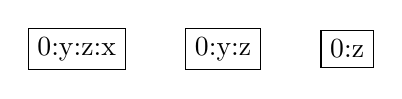
\begin{tikzpicture}[baseline=-2pt]
\node[draw] (phi16_ref1) { 0:y:z:x };
\node[draw,right=5ex of phi16_ref1] (phi16_ref3) { 0:y:z };
\node[draw,right=5ex of phi16_ref3] (phi16_ref5) { 0:z };
\end{tikzpicture}
&
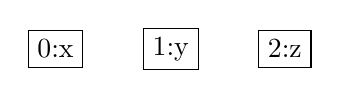
\begin{tikzpicture}[baseline=-2pt]
\node[draw] (phi16_ref2) { 0:x };
\node[draw,right=5ex of phi16_ref2] (phi16_ref4) { 1:y };
\node[draw,right=5ex of phi16_ref4] (phi16_ref6) { 2:z };
\end{tikzpicture}

\\
& \verb~z~ & 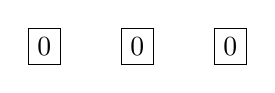
\begin{tikzpicture}[baseline=-2pt]
\node[draw] (pc17ref1) { 0 };
\node[draw,right=5ex of pc17ref1] (pc17ref2) { 0 };
\node[draw,right=5ex of pc17ref2] (pc17ref3) { 0 };
\end{tikzpicture}
&
\begin{tikzpicture}[baseline=-2pt]
\node (d0) {};
\node[draw,right=6em of d0] (pc17ref4) { 2 };
\end{tikzpicture}
\begin{tikzpicture}[overlay]
\draw[->,thick,black] (pc17ref1) edge (phi16_ref1);
\draw[->,thick,black] (pc17ref2) edge (phi16_ref3);
\draw[->,thick,black] (pc17ref3) edge (phi16_ref5);
\draw[->,thick,black] (pc17ref4) edge (phi16_ref6);
\end{tikzpicture}
\\
& \verb~y~ & 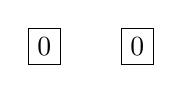
\begin{tikzpicture}[baseline=-2pt]
\node[draw] (pc18ref1) { 0 };
\node[draw,right=5ex of pc18ref1] (pc18ref2) { 0 };
\end{tikzpicture}
&
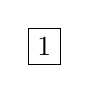
\begin{tikzpicture}[baseline=-2pt]
\node[draw] (pc18ref3) { 1 };
\end{tikzpicture}
\begin{tikzpicture}[overlay]
\draw[->,thick,black] (pc18ref1) edge (pc17ref1);
\draw[->,thick,black] (pc18ref2) edge (pc17ref2);
\draw[->,thick,black] (pc18ref3) edge (phi16_ref4);
\end{tikzpicture}
\\
& \verb~x~ & 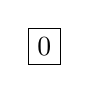
\begin{tikzpicture}[baseline=-2pt]
\node[draw] (pc19ref1) { 0 };
\end{tikzpicture}
&
\begin{tikzpicture}[baseline=-2pt]
\node (d0) {};
\node[draw,left=6em of d0] (pc19ref2) { 0 };
\end{tikzpicture}
\begin{tikzpicture}[overlay]
\draw[->,thick,black] (pc19ref1) edge (pc18ref1);
\draw[->,thick,black] (pc19ref2) edge (phi16_ref2);
\end{tikzpicture}
\\ 
& \verb~y~ & 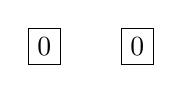
\begin{tikzpicture}[baseline=-2pt]
\node[draw] (pc21ref1) { 0 };
\node[draw,right=5ex of pc21ref1] (pc21ref2) { 0 };
\end{tikzpicture}
&
\begin{tikzpicture}[baseline=-2pt]
\node (d) {};
\node[draw,right=6em of d] (pc21ref3) { 1 };
\end{tikzpicture}
\begin{tikzpicture}[overlay]
\draw[->,thick,black] (pc21ref1) edge (pc19ref1);
\draw[->,thick,black] (pc21ref2) edge (pc18ref2);
\draw[->,thick,black] (pc21ref3) edge (pc18ref3);
\end{tikzpicture}
\\
& \verb~(= z y)~ & 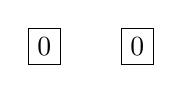
\begin{tikzpicture}[baseline=-2pt]
\node[draw] (pc22ref1) { 0 };
\node[draw,right=5ex of pc22ref1] (pc22ref2) { 0 };
\end{tikzpicture}
&
\begin{tikzpicture}[baseline=-2pt]
\node (d) {};
\node[draw,right=6em] (pc22ref3) { 1 };
\end{tikzpicture}
\begin{tikzpicture}[overlay]
\draw[->,thick,black] (pc22ref1) edge (pc21ref1);
\draw[->,thick,black] (pc22ref2) edge (pc21ref2);
\draw[->,thick,black] (pc22ref3) edge (pc21ref3);
\end{tikzpicture}
\\
& \verb~x~ & 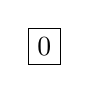
\begin{tikzpicture}[baseline=-2pt]
\node[draw] (pc24ref1) { 0 };
\end{tikzpicture}
&
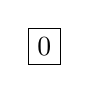
\begin{tikzpicture}[baseline=-2pt]
\node[draw] (pc24ref2) { 0 };
\end{tikzpicture}
\begin{tikzpicture}[overlay]
\draw[->,thick,black] (pc24ref1) edge (pc22ref1);
\draw[->,thick,black] (pc24ref2) edge (pc19ref2);
\end{tikzpicture}
\\
& \verb~(= y x)~ & 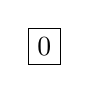
\begin{tikzpicture}[baseline=-2pt]
\node[draw] (pc25ref1) { 0 };
\end{tikzpicture}
&
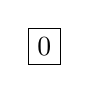
\begin{tikzpicture}[baseline=-2pt]
\node[draw] (pc25ref2) { 0 };
\end{tikzpicture}
\begin{tikzpicture}[overlay]
\draw[->,thick,black] (pc25ref1) edge (pc24ref1);
\draw[->,thick,black] (pc25ref2) edge (pc24ref2);
\end{tikzpicture}
\\
& \verb~(new)~ & \begin{tikzpicture}[baseline=-2pt]
\end{tikzpicture}
&
\begin{tikzpicture}[baseline=-2pt]
\node (d) {};
\node[draw,left=6em of d] (pc30ref1) { 0 };
\end{tikzpicture}
\begin{tikzpicture}[overlay]
\end{tikzpicture}
\\
& \verb~(= x (new))~ & \begin{tikzpicture}[baseline=-2pt]
\end{tikzpicture}
&
\begin{tikzpicture}[baseline=-2pt]
\node (d) {};
\node[draw,left=6em of d] (pc31ref1) { 0 };
\end{tikzpicture}
\begin{tikzpicture}[overlay]
\draw[->,thick,black] (pc31ref1) edge (pc30ref1);
\end{tikzpicture}
\\
& \verb~z~ & 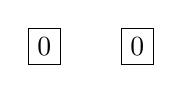
\begin{tikzpicture}[baseline=-2pt]
\node[draw] (pc172ref1) { 0 };
\node[draw,right=5ex of pc172ref1] (pc172ref2) { 0 };
\end{tikzpicture}
&
\begin{tikzpicture}[baseline=-2pt]
\node (d0) {};
\node[draw,right=6em of d0] (pc172ref4) { 2 };
\end{tikzpicture}
\begin{tikzpicture}[overlay]
\draw[->,thick,black] (pc172ref1) edge (pc25ref1);
\draw[->,thick,black] (pc172ref2) edge (pc22ref2);
\draw[->,thick,black] (pc172ref4) edge (pc22ref3);
\end{tikzpicture}
\\
& \verb~y~ & 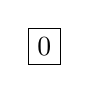
\begin{tikzpicture}[baseline=-2pt]
\node[draw] (pc182ref1) { 0 };
\end{tikzpicture}
&
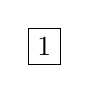
\begin{tikzpicture}[baseline=-2pt]
\node[draw] (pc182ref3) { 1 };
\end{tikzpicture}
\begin{tikzpicture}[overlay]
\draw[->,thick,black] (pc182ref1) edge (pc172ref1);
\draw[->,thick,black] (pc182ref3) edge (pc25ref2);
\end{tikzpicture}
\\
& \verb~x~ & \begin{tikzpicture}[baseline=-2pt]
\end{tikzpicture}
&
\begin{tikzpicture}[baseline=-2pt]
\node (d0) {};
\node[draw,left=6em of d0] (pc192ref2) { 0 };
\end{tikzpicture}
\begin{tikzpicture}[overlay]
\draw[->,thick,black] (pc192ref2) edge (pc31ref1);
\end{tikzpicture}
\\ 
 & \verb~(gotoifnot (! ?) 2)~ & \begin{tikzpicture}[baseline=-2pt]
\end{tikzpicture}
&
\\
& \verb~1:~ & 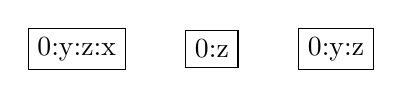
\begin{tikzpicture}[baseline=-2pt]
\node[draw] (phi36_ref1) { 0:y:z:x };
\node[draw,right=5ex of phi36_ref1] (phi36_ref5) { 0:z };
\node[draw,right=5ex of phi36_ref5] (phi36_ref6) { 0:y:z };
\end{tikzpicture}
&
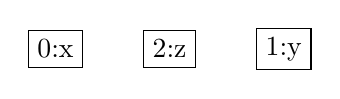
\begin{tikzpicture}[baseline=-2pt]
\node[draw] (phi36_ref2) { 0:x };
\node[draw,right=5ex of phi36_ref2] (phi36_ref3) { 2:z };
\node[draw,right=5ex of phi36_ref3] (phi36_ref4) { 1:y };
\end{tikzpicture}
\\
\end{tabular}
%\end{document}
}
\end{minipage}
\caption{Example of alias trees with generation counting}
On the leftmost column is a simple loop allocating one new object per iteration and keeping it alive for 3 consecutive iterations. It is followed by the lowered representation of the body of the loop, lightly edited for clarity. We expanded the 3 variables two times to make the aliasing and the generation increases more evident.

On the right are the two alias trees corresponding to the two allocation sites. They are automatically generated from our analysis results. The numbers labeling each node are generation numbers. Nodes with explicit variable names are part of an EBB's head summary (our ``$\phi$'' nodes).
\end{figure}



\subsection*{Object fields}

The full abstract heap model with object field is a graph where nodes are labelled with sets of variable definitions and edges with field indices.
We will describe most of the abstract semantic assuming a single field name for simplicity, but the extension to a finite number field names is straightforward.
Adding object fields also implies the presence of summary nodes. They are necessary to avoid infinite increasing chain in the lattice of shape graphs.
A summary node is a node that no local variable points to, and may represent several concrete objects.
There are a lot of different techniques and heuristics on when to collapse empty nodes into summary nodes.
To preserve a fast implementation, we enforce the property that there can be no edge between two summary nodes: we always collapse them together.
This limits the language of heap path we can describe outside our local stack frame to regular expressions of the form $(f_1+\dots+f_n)^*$ where the $f_i$ are field names.

We can define the ordering on this lattice in the following way.
We will say that $H\leq H'$ iff $H$ can be obtained from $H'$ by a succession of moves among those possibilities:
\begin{itemize}
\item Remove a node and all its inbound and outbound edges
\item Remove an edge
\item Split a summary node into two summary nodes and duplicate all edges accordingly
\item Demote a summary node to a normal node
\end{itemize}

\begin{figure}
\centering
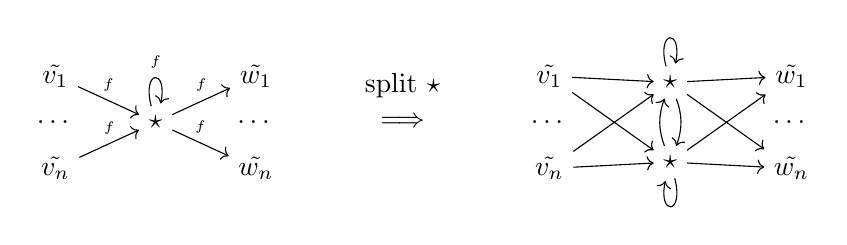
\begin{tikzpicture}
\node (sum) {$\star$};
\node[left=2em of sum] (ldot) {$\dots$};
\node[above=0.5em of ldot] (lv1) {$\tilde{v_1}$};
\node[below=0.5em of ldot] (lvn) {$\tilde{v_n}$};
\node[right=2em of sum] (rdot) {$\dots$};
\node[above=0.5em of rdot] (rv1) {$\tilde{w_1}$};
\node[below=0.5em of rdot] (rvn) {$\tilde{w_n}$};
\draw (lv1) edge[->] node[above]{\tiny$f$} (sum)
      (lvn) edge[->] node[above]{\tiny$f$} (sum)
      (sum) edge[->,loop above] node[above]{\tiny$f$} (sum)
      (sum) edge[->] node[above]{\tiny$f$} (rv1)
      (sum) edge[->] node[above]{\tiny$f$} (rvn);

\node[right=of rdot] (splt) {$\implies$};
\node[above=0em of splt] (spltlbl) {split $\star$};

\node[right=of splt] (ldot2) {$\dots$};
\node[right=3em of ldot2] (sum2) {};
\node[above=0.5em of sum2] (sum21) {$\star$};
\node[below=0.5em of sum2] (sum22) {$\star$};
\node[above=0.5em of ldot2] (lv21) {$\tilde{v_1}$};
\node[below=0.5em of ldot2] (lv2n) {$\tilde{v_n}$};
\node[right=3em of sum2] (rdot2) {$\dots$};
\node[above=0.5em of rdot2] (rv12) {$\tilde{w_1}$};
\node[below=0.5em of rdot2] (rvn2) {$\tilde{w_n}$};
\draw (lv21) edge[->] (sum21)
      (lv2n) edge[->] (sum21)
      (lv21) edge[->] (sum22)
      (lv2n) edge[->] (sum22)
      (sum21) edge[->] (rv12)
      (sum21) edge[->] (rvn2)
      (sum22) edge[->] (rv12)
      (sum22) edge[->] (rvn2)
      (sum21) edge[->,loop above] (sum21)
      (sum22) edge[->,loop below] (sum22)
      (sum21) edge[->,bend left=20] (sum22)
      (sum21) edge[<-,bend right=20] (sum22);
\end{tikzpicture}
\caption{Summary node splitting}
\end{figure}

Most transfer operators on the abstract heap are straightforward. Variable assignments do not change from the simpler model exposed in the last section.
Field assignments are always strong except when the source is a summary node.

We can improve on the naive field access transfer by taking into account incompatible objects.
Assuming no summary nodes, we can describe field access by
\begin{align*}
&E(x,f) = \left\{ x\tilde{u}\to\tilde{v} \in H_{\text{edges}} \right\}
\ \ \ \ \ \ 
N(x,f) = \left\{ \dest(e) ~\middle|~ e \in E(x,f) \right\} \\
&P(y,x,f,\tilde{u}) = \left\{ \tilde{v} \in N(x,f) ~\middle|~ \tilde{v} \cap \tilde{u} = \emptyset\right\} \\
&T[y=x.f](H)_{\text{nodes}} = \big( H_{\text{nodes}} - N(x,f) \big) \cup \bigcup_{\tilde{v}\in N(x,f)} P(y,x,f,\tilde{v}) \cup \left\{ \tilde{v}y \right\} \\
&T[y=x.f](H)_{\text{edges}} = \big( H_{\text{edges}} - E(x,f)\big) \cup \left\{ \src(e)\to\dest(e)y ~\middle|~ e \in E(x,f) \right\}
\end{align*}

\begin{figure}[htpd]
\centering
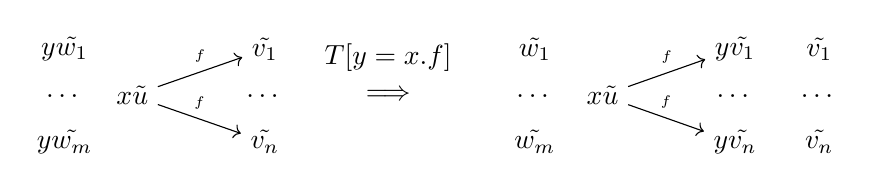
\begin{tikzpicture}
\node[] (xu) {$x\tilde{u}$};
\node[right=of xu] (vdot) {$\dots$};
\node[above=0.5em of vdot] (v1) {$\tilde{v_1}$};
\node[below=0.5em of vdot] (vn) {$\tilde{v_n}$};

\node[left=0.5em of xu] (wdot) {$\dots$};
\node[above=0.5em of wdot] (w1) {$y\tilde{w_1}$};
\node[below=0.5em of wdot] (wn) {$y\tilde{w_m}$};

\draw (xu) edge[->] node[above]{\tiny$f$} (v1)
      (xu) edge[->] node[above]{\tiny$f$} (vn);

\node[right=2em of vdot] (trans) {$\implies$};

\node[above=0em of trans] (translbl) {$T[y=x.f]$};

\node[right=of trans] (wdot2) {$\dots$};
\node[above=0.5em of wdot2] (w12) {$\tilde{w_1}$};
\node[below=0.5em of wdot2] (wn2) {$\tilde{w_m}$};

\node[right=0.5em of wdot2] (xu2) {$x\tilde{u}$};
\node[right=of xu2] (vdot2) {$\dots$};
\node[right=1em of vdot2] (vdot3) {$\dots$};
\node[above=0.5em of vdot2] (v12) {$y\tilde{v_1}$};
\node[below=0.5em of vdot2] (vn2) {$y\tilde{v_n}$};
\node[above=0.5em of vdot3] (v13) {$\tilde{v_1}$};
\node[below=0.5em of vdot3] (vn3) {$\tilde{v_n}$};
\draw (xu2) edge[->] node[above]{\tiny$f$} (v12)
      (xu2) edge[->] node[above]{\tiny$f$} (vn2);
\end{tikzpicture}

\ 

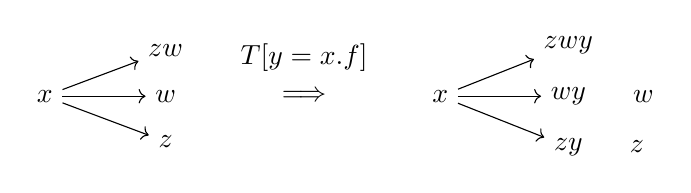
\begin{tikzpicture}
\node (x) {$x$};
\node[right=3em of x] (bl) {$w$};
\node[above=0.5em of bl] (zw) {$zw$};
\node[below=0.5em of bl] (z) {$z$};
\draw (x) edge[->] (zw)
      (x) edge[->] (z)
      (x) edge[->] (bl);
\node[right=of bl] (trans) {$\implies$};
\node[above=0em of trans] (translbl) {$T[y=x.f]$};
\node[right=of trans] (x2) {$x$};
\node[right=3em of x2] (bl2) {$wy$};
\node[above=0.5em of bl2] (zw2) {$zwy$};
\node[below=0.5em of bl2] (z2) {$zy$};
\node[right=1em of bl2] {$w$};
\node[right=1em of z2] {$z$};
\draw (x2) edge[->] (zw2)
      (x2) edge[->] (z2)
      (x2) edge[->] (bl2);
\end{tikzpicture}
\caption{Transfer function for field access}
The first graph shows the general case. The second is an example demonstrating incompatible nodes.
\end{figure}


\paragraph{Implementation} Object fields are additional edges in the alias tree, labelled with a field index.
Given an initial segment $x_1\dots x_n$ of the forest, we define the possible values of its $k$th field to be the set of destination of $k$-edges originating at $x_p$ where $p$ is the largest index such that $x_p$ has at least one $k$-edge.
Given this description, translating the abstract transfer into an implementation over the forest is straightforward.

When summarizing the alias tree, we collect fields set during the summarized segment of code and copy those in the EBB head.
This is also the only operation that can introduce new empty nodes. We promote them into summary nodes and merge connected ones.

\subsection*{Context sensitivity}

All the preceding discussion only describes an intraprocedural setting.
Making a heap analysis scale well interproceduraly is challenging.
The most straightforward way of introducing context sensitivity is through \emph{heap cloning}.
Although it has been demonstrated that heap cloning can scale very well\cite{heapclone}, this result is only in the context of a flow-insensitive analysis.

We make the choice not to introduce any context sensitive information while computing the fixpoint of the abstract heap over a function.
In the setting we described until now, we would have to treat function arguments -- and objects reachable from them -- conservatively as a single summary node.
We instead introduce a new type of node that tries to keep more information by being less pessimistic about aliasing.
Of course, inside the callee, we still can't answer the question whether those outside objects alias or not.
However, by keeping them separated we allow the caller to regain some information by eliminating impossible nodes and perform a form of ``post-facto context sensitivity'' using call site information.

This new type of node, that we will call \emph{context} nodes, do not have the guarantee not to alias each other.
Unlike summary nodes however, each is still mapped to at most a single concrete object.
We will note context nodes by prefixing their content with $\gamma$.
We include context nodes in the abstract semantic by adding the following rule to the set of $H\leq H'$ moves previously described.

One can contract ($\kappa$) two context nodes.
The label of the resulting node is the union of the two labels.
Edges from and to the nodes must be duplicated for every element of the cartesian product of the source and destination nodes respectively.
More precisely, still assuming a single field name for clarity, the contraction of two $\gamma$ nodes can be expressed as
\[
*\to\gamma\tilde{u} = \left\{ e \in H_{\text{edges}} ~\middle|~ \dest(e) = \gamma\tilde{u} \right\}
\ \ \ \ \ 
\gamma\tilde{u}\to * = \left\{ e \in H_{\text{edges}} ~\middle|~ \src(e) = \gamma\tilde{u} \right\} 
\]
\begin{align*}
&\kappa[\gamma\tilde{u},\gamma\tilde{v}](H)_{\text{nodes}} = &\ \big( H_{\text{nodes}} - \left\{\gamma\tilde{u}, \gamma\tilde{v}\right\} \big) \cup \left\{ \gamma\tilde{u}\tilde{v} \right\} \\
&&-\ \big( \src(*\to\gamma\tilde{u}) \cup \src(*\to\gamma\tilde{v}) \cup \dest(\gamma\tilde{u}\to *) \cup \dest(\gamma\tilde{v}\to *) \big) \\
&&\cup \left\{ \src(e)\src(e') ~\middle|~ e \in *\to\gamma\tilde{u}, e' \in *\to\gamma\tilde{v} \right\} \\
&&\cup \left\{ \dest(e)\dest(e') ~\middle|~ e \in \gamma\tilde{u}\to *, e' \in \gamma\tilde{v}\to * \right\} \\
&\kappa[\gamma\tilde{u},\gamma\tilde{v}](H)_{\text{edges}} = &\ H_{\text{edges}} - \big( *\to\gamma\tilde{u} \cup *\to\gamma\tilde{v} \cup \gamma\tilde{u}\to * \cup \gamma\tilde{v}\to * \big) \\
&&\cup \left\{ \src(e)\src(e') \to \gamma\tilde{u}\tilde{v} ~\middle|~ e \in *\to\gamma\tilde{u}, e' \in *\to\gamma\tilde{v} \right\} \\
&&\cup \left\{ \gamma\tilde{u}\tilde{v} \to \dest(e)\dest(e') ~\middle|~ e \in \gamma\tilde{u}\to *, e' \in \gamma\tilde{v}\to * \right\} \\
\end{align*}

\begin{figure}[htdp]
\centering
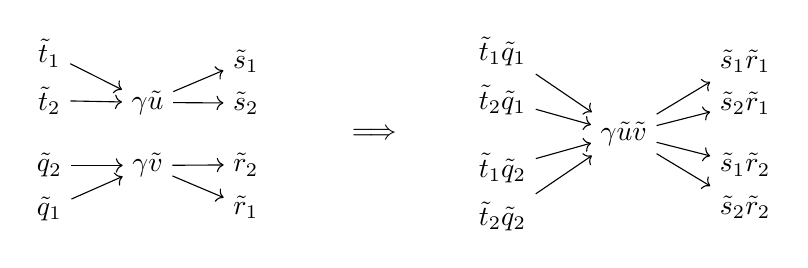
\begin{tikzpicture}
\node (mid1) {};
\node[above=0em of mid1] (u) {$\gamma\tilde{u}$};
\node[below=0em of mid1] (v) {$\gamma\tilde{v}$};
\node[left=of mid1] (inmid) {};
\node[above=0em of inmid] (in2) {$\tilde{t}_2$};
\node[above=0em of in2] (in1) {$\tilde{t}_1$};
\node[below=0em of inmid] (in4) {$\tilde{q}_2$};
\node[below=0em of in4] (in3) {$\tilde{q}_1$};
\node[right=of mid1] (outmid) {};
\node[above=0em of outmid] (out2) {$\tilde{s}_2$};
\node[above=0em of out2] (out1) {$\tilde{s}_1$};
\node[below=0em of outmid] (out4) {$\tilde{r}_2$};
\node[below=0em of out4] (out3) {$\tilde{r}_1$};
\draw (in1) edge[->] (u)
      (in2) edge[->] (u)
      (in3) edge[->] (v)
      (in4) edge[->] (v);
\draw (out1) edge[<-] (u)
      (out2) edge[<-] (u)
      (out3) edge[<-] (v)
      (out4) edge[<-] (v);
\node[right=of outmid] (kap) {$\implies$};
\node[above=0em of kap] (kaplbl) {$\kappa$};
\node[right=of kap] (inmid2) {};
\node[right=of inmid2] (uv) {$\gamma\tilde{u}\tilde{v}$};
\node[above=0em of inmid2] (in21) {$\tilde{t}_2\tilde{q}_1$};
\node[above=0em of in21] (in22) {$\tilde{t}_1\tilde{q}_1$};
\node[below=0em of inmid2] (in23) {$\tilde{t}_1\tilde{q}_2$};
\node[below=0em of in23] (in24) {$\tilde{t}_2\tilde{q}_2$};

\node[right=of uv] (outmid2) {};
\node[above=0em of outmid2] (out21) {$\tilde{s}_2\tilde{r}_1$};
\node[above=0em of out21] (out22) {$\tilde{s}_1\tilde{r}_1$};
\node[below=0em of outmid2] (out23) {$\tilde{s}_1\tilde{r}_2$};
\node[below=0em of out23] (out24) {$\tilde{s}_2\tilde{r}_2$};
\draw (in21) edge[->] (uv)
      (in22) edge[->] (uv)
      (in23) edge[->] (uv)
      (in24) edge[->] (uv);
\draw (out21) edge[<-] (uv)
      (out22) edge[<-] (uv)
      (out23) edge[<-] (uv)
      (out24) edge[<-] (uv);

\end{tikzpicture}
\caption{Contraction of two context nodes}
\end{figure}

An interesting consequence of this choice of semantic is that we can still perform strong field updates on $\gamma$ nodes.
They are weaker than local nodes in the two following ways:
\begin{itemize}
\item Other part of the interpreter cannot assume that two different $\gamma$ nodes don't alias.
\item The field access of a $\gamma$ node is weaker.
\end{itemize}

The only change we need to make to $T[y=x.f]$ when $x$ is part of a $\gamma$ node is that we have to keep edges between $\gamma x\dots$ and the dangling nodes $\tilde{v}_i$ introduced.

Checking 


\section*{I can see the future}

[summary of contributions] [technical/impl things] [backward analysis?]

\paragraph{Generic sparsification} We hypothesize that a general transform from dense to sparse state structure underlies the particular one presented in this report and included in our implementation.
Although we do not hope for a fully mechanized way to do such a conversion, it is likely that we could provide a set of generic reusable component to make the implementation as well as the soundness proof of those state domains easier.
As more use cases appear we will try to develop a general framework, both theoretical and implementation-wise, for this process.

\paragraph{User provided optimizations} We briefly hinted at domain-specific optimizations in the introduction.
Our long term plan is to provide hooks in the compiler and the analyzer to allow for user defined analysis and optimization.
Moreover, those should be able to easily build upon the existing infrastructure.
Although the abstract interpreter model is a good fit in that regard, we have not yet found a fully satisfactory equivalent for the optimization side.

As a good example of the envisioned usefulness of this kind of modularity, consider the development of a high-level interface to a BLAS library.
This was not chosen at random since the linear algebra routines are in fact a sizable chunk of the Julia standard library, and BLAS is used as their back end in the common case floating point numeric types.

It is easy to use under a simple model where the output of the computation is freshly allocated memory containing the result. This avoids aliasing bugs, however it is inefficient because it does not take advantage of the specialized BLAS functions that can output the result in place. Reasoning that the two are equivalent if one of the argument (and all its aliases) are dead after the BLAS call is almost impossible to the compiler because it requires understanding of the routine, of which the core is often hand written assembly.
However, the rules of BLAS aliasing are very regular at a high level and someone writing a wrapper for the library could easily, given the right interface, integrate those rules directly as a compiler extension.

As we work towards making the interpreter more accessible, the need for good tooling becomes unavoidable.

\paragraph{Abstract debugging} We would like to provide a common infrastructure aimed at debugging abstract domains.
In its simplest form, this system would open the possibility for a domain to provide small run-time guards checking that the state conforms to what was inferred.
The analyzer would then, in ``verification'' mode, insert those guards in the code before running it, along with the necessary information to trace back the exact transfer function that computed an unsound result.
This would obviously not replace a formal proof of soundness but would help weed out implementation errors by large scale testing on the consequent amount of freely available Julia source.

\paragraph{Visualization} As a way to help implementation work, a graphical visualization of the interpreter was hastily put together.
The usefulness of this tool exceeded our -- admittedly low -- expectations. [maybe screenshot in annex]
We believe that interactive feedback is a key aspect of allowing users with no particular background in program analysis to develop an understanding of the -- in fact quite natural -- underlying model.

\newpage

\begin{thebibliography}{9}
\bibitem[Lat02]{llvm} Chris Lattner -- \emph{LLVM: An Infrastructure for Multi-Stage Optimization} (M.S. Thesis, University of Illinois, 2002)
\bibitem[GAE09]{js-trace} Gal, Andreas, Brendan Eich, Mike Shaver, David Anderson, David Mandelin, Mohammad R. Haghighat, Blake Kaplan et al -- \emph{Trace-based just-in-time type specialization for dynamic languages} (ACM 2009)
\bibitem[BEK14]{julia-paper} Jeff Bezanson, Alan Edelman, Stefan Karpinski, Viral B. Shah -- \emph{Julia: A fresh approach to numerical computing} (2014) \verb~arXiv:1411.1607~
\bibitem[BAP86]{cl} Brooks, Rodney A., David B. Posner, James L. McDonald, Jon L. White, Eric Benson, and Richard P. Gabriel -- \emph{Design of an optimizing, dynamically retargetable compiler for common Lisp} (ACM 1986)
\bibitem[SMR98]{ssc} Sagiv, Mooly, Thomas Reps, Reinhard Wilhelm -- \emph{Solving shape-analysis problems in languages with destructive updating} (TOPLAS 1998)
\bibitem[CC77]{absint-cousot} Patrick Cousot, Radhia Cousot -- \emph{Abstract interpretation: a unified lattice model for static analysis of programs by construction or approximation of fixpoints} (SIGPLAN 1977)
\bibitem[CCM11]{redprod} Patrick Cousot, Radhia Cousot, Laurent Mauborgne -- \emph{The reduced product of abstract domains and the combination of decision procedures} (Foundations of Software Science and Computational Structures, 2011)
\bibitem[Bez15]{jeff-phd} Jeff Bezanson -- \emph{Abstraction in Technical Computing} (2015)
\bibitem[LoA15]{ssa-book} ``Lots of authors'' -- \emph{Static Single Assignment Book} (2015)
\bibitem[NL09]{ssa-alias} N. A. Naeem, O. Lhotak -- \emph{Efficient alias set analysis using SSA form} (ISMM 2009)
\bibitem[OHL12]{sparse-nr} Hakjoo Oh, Kihong Heo, Wonchan Lee, Woosuk Lee, Kwangkeun Yi -- \emph{Design and Implementation of Sparse Global Analyses for C-like Languages} (PLDI 2012)
\bibitem[CDH01]{domtree} Cooper, Keith D., Timothy J. Harvey, Ken Kennedy -- \emph{A simple, fast dominance algorithm} (2001)
\bibitem[LLA07]{heapclone} Chris Lattner, Andrew Lenharth, Vikram Adve -- \emph{Making context-sensitive points-to analysis with heap cloning practical for the real world} (SIGPLAN 2007)
\bibitem{julia-web} \verb~http://julialang.org~
\bibitem{gf-web} \verb~https://github.com/carnaval/green-fairy~
\end{thebibliography}

\end{document}
